\lstinputlisting[language=bash,basicstyle=\small]{python_codes/fieldstone_31/keywords.ascii}

\begin{center}
Code at \url{https://github.com/cedrict/fieldstone/tree/master/python_codes/fieldstone_31}
\end{center}

\par\noindent\rule{\textwidth}{0.4pt}
%%%%%%%%%%%%%%%%%%%%%%%%%%%%%%%%%%%%%%%%%%%%%%%%%%%%%%%%%%%%%%%%%%%%%%%%%%%%%%%%%%%%%%%%%%%%


This benchmark begins by postulating a polynomial solution to the 3D Stokes equation:
\begin{equation}
{\bm v}
=
\left(
\begin{array}{c}
(y+z)(1-x^2) \\
(-x+z)(1-y^2) \\
(-x-y)(1-z^2) 
\end{array}
\right)
\label{eqgarf}
\end{equation}
Let us compute all the strain rate tensor components:
\begin{eqnarray}
\dot{\epsilon}_{xx}&=& -2x(y+z)  \nonumber\\
\dot{\epsilon}_{yy}&=& -2y(-x+z) \nonumber\\
\dot{\epsilon}_{zz}&=& -2z(-x-z)) \nonumber\\
2 \dot{\epsilon}_{xy}&=& \frac{1}{2}(y^2-x^2) \nonumber\\ 
2 \dot{\epsilon}_{xz}&=& \frac{1}{2}(z^2-x^2)  \nonumber\\
2 \dot{\epsilon}_{yz}&=& \frac{1}{2}(y^2-y^2)  \nonumber
\end{eqnarray}
In passing, one can verify that 
$
\dot{\epsilon}_{xx}
+\dot{\epsilon}_{yy}
+\dot{\epsilon}_{zz}=0
$.

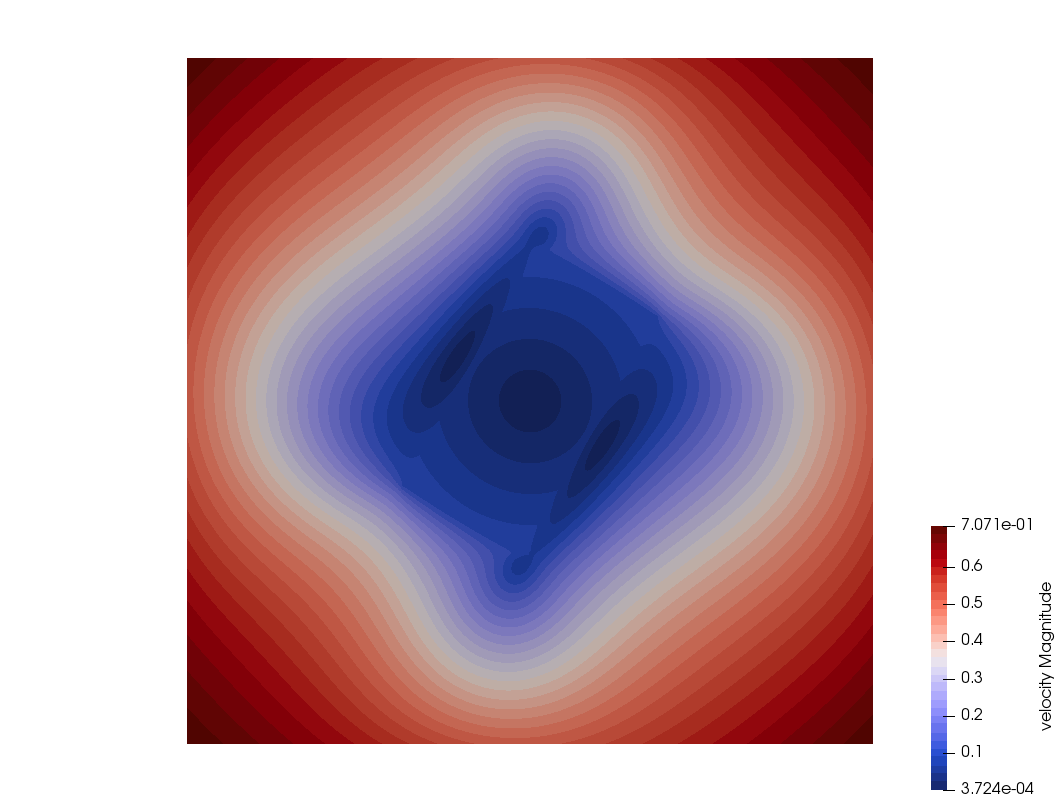
\includegraphics[width=7cm]{python_codes/fieldstone_31/vel1}
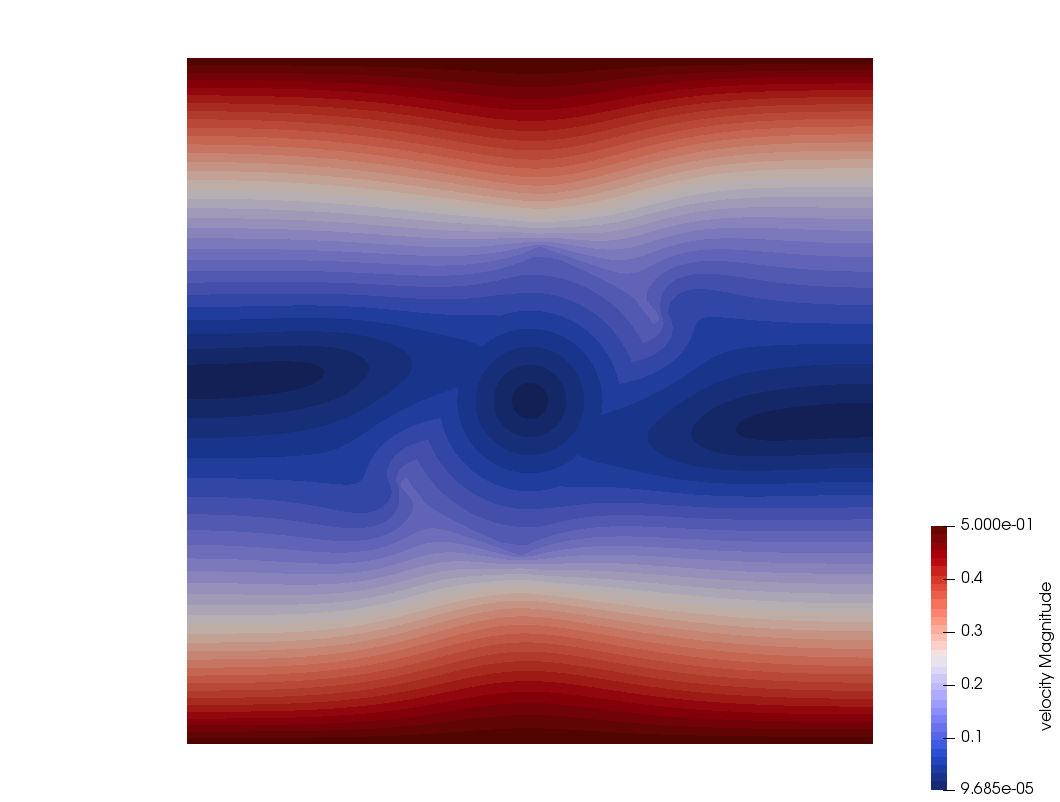
\includegraphics[width=7cm]{python_codes/fieldstone_31/vel2}





